\documentclass[10pt,conference,a4paper]{IEEEtran}
%\documentclass[12pt,draftcls,twocolumn]{IEEEtran}
\usepackage{ifpdf}
%\usepackage{cite}
\usepackage{subfig}
\pagestyle{plain}




% *** GRAPHICS RELATED PACKAGES ***
%
\ifCLASSINFOpdf
  \usepackage[pdftex]{graphicx}
  % declare the path(s) where your graphic files are
  \graphicspath{{../pdf/}{../jpeg/}}
  % and their extensions so you won't have to specify these with
  % every instance of \includegraphics
  \DeclareGraphicsExtensions{.pdf,.jpeg,.png}
\else
  % or other class option (dvipsone, dvipdf, if not using dvips). graphicx
  % will default to the driver specified in the system graphics.cfg if no
  % driver is specified.
  \usepackage[dvips]{graphicx}
  % declare the path(s) where your graphic files are
  \graphicspath{{../eps/}}
  % and their extensions so you won't have to specify these with
  % every instance of \includegraphics
  \DeclareGraphicsExtensions{.eps}
  \fi
%  \DeclareMathOperator{\vecOp}{\mathrm{vec}}
%	\DeclareMathOperator{\tr}{\mathrm{tr}}
%	\DeclareMathOperator{\E}{\mathbb{E}}
%	\DeclareMathOperator{\var}{\mathbb{V}\mathrm{ar}}
%	\DeclareMathOperator{\cov}{\mathrm{Cov}}
%	\DeclareMathOperator{\sgn}{\mathrm{sgn}}
%	\DeclareMathOperator{\etr}{\mathrm{etr}}
%	\DeclareMathOperator{\re}{\mathfrak{Re}}
%	\DeclareMathOperator{\im}{\mathfrak{Im}}
%\documentclass[10pt,conference,a4paper,compsocconf]{IEEEtran}
%\documentclass[11pt]{article}
%\usepackage{graphicx}
%\usepackage{amsmath,amssymb,hyperref,fancyhdr}%fancyhdr
\usepackage{amsmath,amsxtra,amssymb,amsthm,latexsym,amscd,amsfonts}
%\usepackage[utf8]{vietnam}
\usepackage[utf8]{vntex}
%\usepackage{fancyhdr}
%\pagestyle{fancy}
\renewcommand{\sectionmark}[1]{\markright{\MakeUppercase{#1}}{}}
%\renewcommand{\headrulewidth}{0pt}
\ifCLASSINFOpdf
\usepackage[pdftex]{graphicx}
\DeclareGraphicsExtensions{.pdf,.jpeg,.png,.jpg}
\else
\usepackage[dvips]{graphicx}
\DeclareGraphicsExtensions{.eps}
\fi
\usepackage{array}
\usepackage{epstopdf}
%\usepackage[font=footnotesize]{subfig}
%\hyphenation{op-tical net-works semi-conduc-tor}
\usepackage{anysize}
%\marginsize{2.4cm}{2.0cm}{3.8cm}{3.6cm}
% Use other margin values if the pdf file does not fit the word template (left: 2.4cm, right: 2.0cm, top: 3.8cm, bottom: 3.6cm)
\marginsize{2.4cm}{2.0cm}{3.2cm}{3.0cm}
%\marginsize{2.4cm}{1.4cm}{2.4cm}{2cm}
\usepackage{multicol}
\usepackage{balance}

\hyphenation{op-tical net-works semi-conduc-tor}
\newtheorem{theorem}{Theorem}
\newtheorem{lemma}[theorem]{Lemma}
%\newtheorem{proposition}[theorem]{Proposition}
\newtheorem{corollary}[theorem]{Corollary}
\newtheorem{proposition}{Bổ Đề}

\makeatletter
\def\ScaleIfNeeded{\ifdim\Gin@nat@width>\linewidth\linewidth\else\Gin@nat@width\fi}

\begin{document}
\columnsep=0.63cm
%---Mathematical symbols ------------------------------------------------------
\def\mathbi#1{\boldsymbol{#1}}
\def\erfc{\:\mathrm{erfc}}
\def\arg{\:\mathrm{arg}}
\def\E{\:\mathrm{E}}
\def\sinc{\:\mathrm{sinc}}
\def\T{\mathrm{T}}
\def\H{\mathrm{H}}
\newcommand{\bigsize}{\fontsize{16pt}{20pt}\selectfont}

%
% paper title
% can use linebreaks \\ within to get better formatting as desired

\include{Abbr}
\title{Ứng dụng Xử lý ảnh và Machine Learning để nhận dạng và phân loại xe 2 bánh và 4 bánh trong video }

\author{
\IEEEauthorblockN{
	Nguyễn Huỳnh Đức\IEEEauthorrefmark{1}
Nguyễn Hồng Hưng\IEEEauthorrefmark{1},
Nguyễn Hoàng Phúc\IEEEauthorrefmark{1}
Văn Đình Triều\IEEEauthorrefmark{1}
Lê Tuấn Vũ\IEEEauthorrefmark{1} 
} 
\IEEEauthorblockA{\IEEEauthorrefmark{1} Lớp Viễn thông - PFIEV - 2014 \\ Đại học Bách Khoa Thành Phố Hồ Chí Minh \\ Môn học: Xử lý số hình ảnh và âm thanh - GVHD: ThS. Đặng Nguyên Châu\\
		Email: \{1510797,1411608, 1412957, 1414177, 1414741\}@hcmut.edu.vn}
}
\maketitle


\begin{abstract}
%\boldmath 
Trong bài báo này, nhóm ứng dụng những kiến thức đã học về xử lý ảnh, cũng như tìm hiểu về một số giải thuật phân lớp để loại các vật thể. Nhóm áp dụng kĩ thuật trích xuất đặc trưng HOG (Histogram of Oriented Gradient) và phương pháp phân lớp (classification)  SVM (Support Vector Machine) để  nhận dạng các vật thể trong một video. Nhóm đã tiến hành thực nghiệm nhận dạng và phân loại xe 2 bánh và xe 4 bánh, kết quả đạt được có độ chính xác khá tốt.
	 
\end{abstract}

\begin{IEEEkeywords}
Digital Image Processing, Classification, Histogram of Oriented Gradient, Support Vector Machine, Vehicle Detection.
\end{IEEEkeywords}
\IEEEpeerreviewmaketitle
%
\section{GIỚI THIỆU}
%
Phân loại ảnh là một bài toán đã và đang thu hút được sự quan tâm của các nhà nghiên cứu và phát triển, được ứng dụng rộng rãi nhiều ứng dụng hữu ích như: tìm kiếm ảnh, nhận dạng, theo dõi và phát hiện đối tượng... Trong giám sát đối tượng chuyển động từ video chẳng hạn như giám sát phương tiện giao thông, thì phân loại ảnh là bài toán kế tiếp sau bài toán phát hiện đối tượng chuyển động.Khi đó bài toán đối sánh ảnh sẽ quy về bài toán so sánh các đặc trưng trích chọn. Các đặc trưng cho phép biểu diễn ảnh đã được nghiên cứu bao gồm đường biên vùng ảnh, điểm ảnh đặc trưng, lược đồ xám (histogram),lược đồ vector gradient (Histogram of Oriented Gradient)... \\
Có hai vấn đề cơ bản thường đặt ra trong bài toán phân loại: i) làm sao có thể biểu diễn thông tin một cách hiệu quả nhằm thực hiện việc đối sánh hai ảnh nhanh nhất có thể; ii) làm thế nào để giải pháp đối sánh vẫn hoạt động hiệu quả khi có sự thay đổi của môi trường: nhiễu trong quá trình thu nhận ảnh, sự thay đổi về ánh sáng, sự che khuất,...


Cùng với sự phát triển của các thuật toán phân loại, các ứng dụng nhận diện có độ chính xác ngày càng gia tăng. Dù không thể bằng con người nhưng kết quả của các phần mềm nhận diện cho thấy khá khả quan với những sai số có thể chấp nhận. Người ta đã ứng dụng các thuật toán phân loại vào rất nhiều đối tượng trong cuộc sống, cụ thể là nhận diện các loại phương tiện giao thông. Với mục đích tìm hiểu về các thuật toán machine learning và phát triển một phần mềm phân loại và nhận diện, nhóm muốn được thử sức về đề tài “Phân loại các loại trong một video” bằng phương pháp trích đặc trưng Histogram of Oriented Gradient (HOG) và phân loại bằng thuật toán Support Vector Machine (SVM). Lý do nhóm sử dụng các kỹ thuật này là nhờ những ưu điểm mà chúng mang lại: HOG giúp mô tả vật thể trong một bức ảnh và SVM giúp tìm ra được mặt phân chia tối ưu trong không gian nhiều chiều. Các báo cáo về SVM trên thế giới cho thấy, SVM cho kết quả phân loại tốt hơn Perceptron Learning Algorithm nhờ mặt phân chia tối ưu. 



Trong các phần tiếp theo của bài báo này, nhóm xin trình bày phương pháp tiếp cận của nhóm. Trong phần~\ref{Sec:soluocgiaithuat} và phần~\ref{Sec:Cacbuocthuchien}, nhóm lần lượt trình bày sơ lược giải thuật và phân tích các bước thực hiện. Trong phần~\ref{Sec:KetQuaMoPhong}, nhóm sẽ kiểm chứng các kết quả phân tích bằng các kết quả mô phỏng trên Python. Cuối cùng, nhóm kết luận bài báo trong phần~\ref{Sec:KetLuan}.
%
\section{SƠ LƯỢC GIẢI THUẬT}
\label{Sec:soluocgiaithuat}
\begin{figure}[ht]
	\centering
	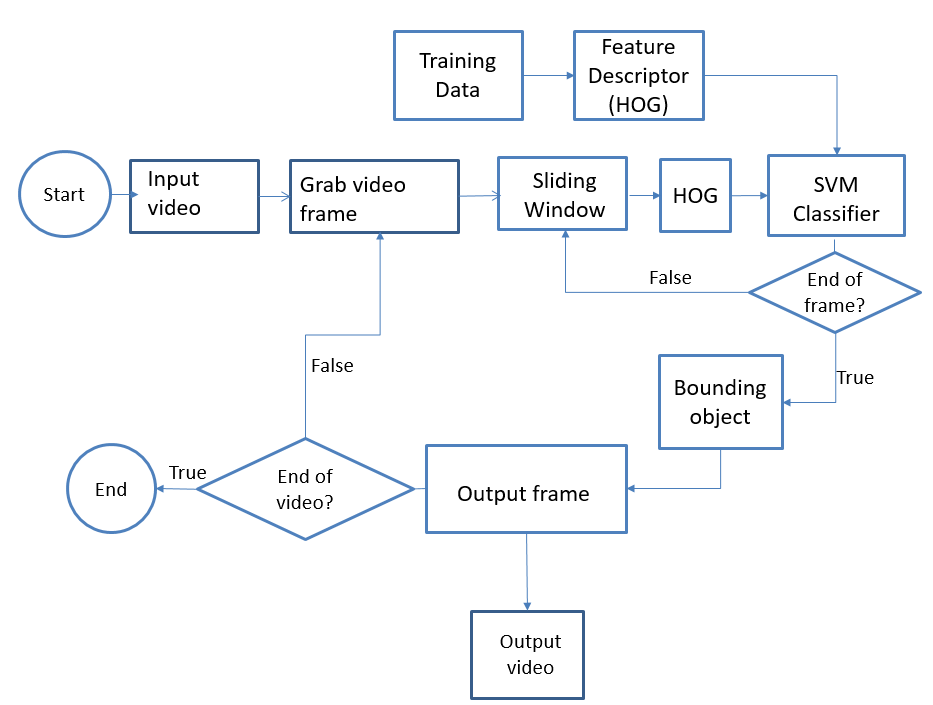
\includegraphics[width=\ScaleIfNeeded]{scheme2}
	\caption{Sơ đồ nguyên lí}
	\label{fig:scheme2}
\end{figure}





Chúng ta xem xét sơ đồ nguyên lí chung được mô tả như trong Hình~\ref{fig:scheme2}, với Input là video đầu vào, ta tách từng frame video ra và xử lí trên từng frame đó. Sau khi thực hiện xong, các frame đã qua xử lý sẽ được lưu lại tại bộ nhớ đệm để tạo thành video mà trong đó các xe 2 bánh và 4 bánh đã được nhận dạng.
Chúng ta sẽ phân tích kĩ hơn ở các khối như trích xuất đặc trưng HOG khối SVM classifier, sliding window, đây là những khối chính của cả sơ đồ. 

	





\section{PHÂN TÍCH CÁC BƯỚC THỰC HIỆN}
\label{Sec:Cacbuocthuchien}
%
\subsection{Histogram of Oriented Gradient}   
HOG(histogram of oriented gradients) là một feature descriptor được sử dụng trong computer vision và xử lý hình ảnh, dùng để detect một đối tượng.\cite{viblo.asia} \cite{learnopencv} \\,
Các khái niệm về HOG được nêu ra từ năm 1986 tuy nhiên cho đến năm 2005 HOG mới được sử dụng rộng rãi sau khi Navneet Dalal và Bill Triggs công bố những bổ sung về HOG. Hog tương tự như các biểu đồ edge orientation, scale-invariant feature transform descriptors(như sift, surf,..), shape contexts nhưng HOG được tính toán trên một lưới dày đặc các cell và chuẩn hóa sự tương phản giữa các block để nâng cao độ chính xác. Hog được sử dụng chủ yếu để trích xuất đặc trưng một object trong ảnh Bài toán tính toán Hog thường gồm 5 bước:
	\begin{itemize}
		\item Chuẩn hóa hình ảnh trước khi xử lý
		\item Tính toán gradient theo cả hướng x và y
		\item Lấy phiếu bầu cùng trọng số trong các cell
		\item Chuẩn hóa các block
		\item Thu thập tất cả các biểu đồ cường độ gradient định hướng để tạo ra feature vector cuối cùng
	\end{itemize}

\subsubsection{Chuẩn hóa hình ảnh trước khi xử lý}
%
Bước chuẩn hóa này hoàn toàn không bắt buộc, nhưng trong một số trường hợp, bước này có thể cải thiện hiệu suất của bộ mô tả HOG. Đối với đề tài này, các hình ảnh đã được đưa về cùng độ phân giải là 64x64 pixels.
\subsubsection{Tính toán gradient theo 2 hướng }
Gradient của một bức hình là 1 vector với 2 thành phần:

\[\nabla f = \left[ {\begin{array}{*{20}{c}}
	{{g_x}}\\
	{{g_y}}
	\end{array}} \right] = \left[ {\begin{array}{*{20}{c}}
	{\frac{{\partial f}}{{\partial {\rm{x}}}}}\\
	{\frac{{\partial f}}{{\partial y}}}
	\end{array}} \right]\]

Với  ${g_x},\,{g_y}$  lần lượt là gradient theo phương x và y. Để tính giá trị gradient, ta tính tính chập $G = I \otimes D$  ,với $I$  là hình ảnh đầu vào,  $ D $ là mặt nạ gradient, hay còn gọi là kernel.Hình dưới đây là một số kernel hay sử dụng.



\begin{figure}[!htp]
	\centering
	\subfloat[Sobel kernel size 1]
	{	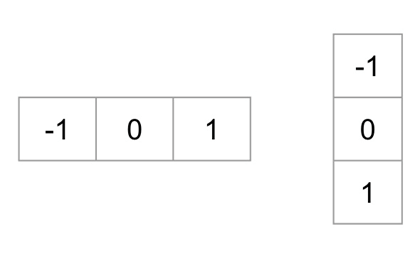
\includegraphics[width=0.7\linewidth]{sobel1}}\hfill
	\centering
	\subfloat[Sobel kernel size 3]
	{	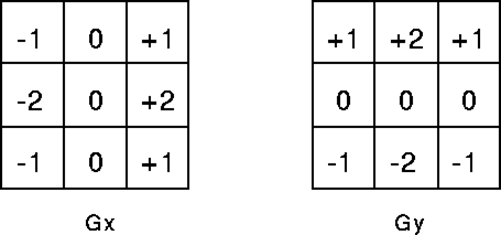
\includegraphics[width=0.7\linewidth]{sobel2}}\hfill
		\centering
	\subfloat[scharr kernel]
	{	\includegraphics[width=\ScaleIfNeeded]{"scharr kernel"}}\hfill
	\caption{Các kernel thông dụng}
	
	
\end{figure}


Sau khi có các giá trị gradient theo phương x và y, ta có thể biểu diễn thành một vector với cường độ là  $g = \sqrt {{g_x}^2 + {g_y}^2} $ , hướng $\theta  = \arctan \left( {\frac{{{g_y}}}{{{g_x}}}} \right)$

Dưới đây là hình mô tả các vector gradient của một bức hình 16x16 pixels, trong đó các ô vuông xanh tượng trưng cho các điểm ảnh, các mũi tên đen là các vector gradient.
  
\begin{figure}[!htp]
	\centering
	\includegraphics[width=\ScaleIfNeeded]{"gradient vector"}
	\caption{Minh hoạ gradient vector của một bức ảnh 16x16 pixels}
	\label{fig:gradient-vector}
\end{figure}

\subsubsection{Lấy phiếu bầu cùng trọng số trong các cell}
Một trong những lý do quan trọng sử dụng HOG đó là chúng ta cần tìm ra đặc trưng của bức ảnh (feature descriptor) một cách súc tích nhất. Do đó thay vì dùng đến 256 vector gradient (ứng với 256 điểm ảnh) để biểu thị một bức ảnh, ta có thể giảm số vector này xuống mà vẫn thể hiện được đặc trưng của bức ảnh đó. Trong bước  này, bức ảnh trên sẽ được chia thành 16 ô vuông, tức 4x4 cells, và tương ứng sẽ chỉ còn 16 vector gradient.
Công việc tiếp theo là ta sẽ lập histogram của gradient cho mỗi cell bằng phương pháp lấy phiếu bầu cùng trọng số trong một cell.

Ví dụ ta có hình dưới đây đã được chia thành các cell, mỗi cell có kích thước 8x8 pixels, sau khi thực hiện bước 2 ta có các giá trị vector gradient (gồm biên độ và hướng) của mỗi pixel.

\begin{figure}[!htp]
	\centering
	\includegraphics[width=\ScaleIfNeeded]{"gradient vector2"}
	\caption{Hình được chia thành các cell 8x8 pixel}
	\label{fig:gradient-vector2}
\end{figure}

Với mỗi cell trong bức ảnh, ta cần xây dựng 1 biểu đồ cường độ gradient. Mỗi pixcel sẽ được vote vào vào biểu đồ, trọng số của mỗi vote chính là cường độ gradient tại pixel đó Cuối cùng, mỗi pixel đóng góp một phiếu bầu có trọng số vào biểu đồ - trọng lượng của phiếu chỉ đơn giản là cường độ gradient |G| tại pixel đó.Lúc này, chúng ta có thể thu thập và ghép các biểu đồ này để tạo ra feature vector cuối cùng.\\
Dựa vào các số liệu này, ta sẽ tạo ra một histogram gồm có 9 mức, ứng với 9 hướng của vectơ gradient : 0, 20, 40 … 160$^\circ $  Hình dưới đây minh hoạ cho quá trình tính toán này.\\
\begin{figure}[ht]
	\centering
	\includegraphics[width=\ScaleIfNeeded]{"histogram gradient"}
	\caption{Quá trình tạo historgram gradient bằng voting}
	\label{fig:histogram-gradient}
\end{figure}



Ô màu xanh biểu thị cho vector gradient có biên độ là 2, góc 80$^\circ $, ở trên thang 80$^\circ $ của histogram ta gán giá trị 2 vào.  
Đối với ô màu đỏ, vector gradient có biên độ 4, góc 10$^\circ $, ở trên thang histogram không có giá trị này, vì vậy nó sẽ vote cho 2 thang gần nhất với  nó, tức là thang 0$^\circ $ và 20$^\circ $. Lưu ý tỉ lệ vote sẽ bằng 1:1 bởi vì giá trị góc của vector là 10$^\circ $, cách đều 2 thang 0$^\circ $ và 20$^\circ $.

\begin{figure}[ht]
	\centering
	\includegraphics[width=\ScaleIfNeeded]{"histogram gradient1"}
	\caption{Histogram gradient calculating}
	\label{fig:histogram-gradient1}
\end{figure}
Một trường hợp khác đó là góc của vector nằm trong khoảng 160$^\circ $ - 180$^\circ $, lúc này ta vẫn làm tương tự như trên, tuy nhiên thay vì vote cho thang 180$^\circ $, ta sẽ vote cho thang 0$^\circ $. Sau khi tổng hợp tất cả các điểm ảnh trong 1 cell, ta được histogram gradient có dạng như hình.\\
Như vậy sau bước 3, số vectơ gradient đặc trưng cho 1 cell giảm từ 64 vector xuống còn 9 vector.
\linebreak
\begin{figure}[ht]
	\centering
	\includegraphics[width=\ScaleIfNeeded]{"histogram gradient2"}
	\caption{Histogram of Gradient}
	\label{fig:histogram-gradient2}
\end{figure}
\subsubsection{Chuẩn hóa các block}


Ở bước trước, chúng ta đã tạo ra một biểu đồ dựa trên gradient của hình ảnh. Gradient của hình ảnh rất nhạy cảm với ánh sáng tổng thể. Nếu hình ảnh được làm cho tối hơn bằng cách chia tất cả các giá trị pixel cho 2, cường độ gradient sẽ thay đổi một nửa và do đó, các giá trị biểu đồ sẽ thay đổi một nửa. Một cách lý tưởng, chúng ta muốn các đặc trưng của một bức hình độc lập với sự thay đổi của độ sáng. Để làm được điều này, chúng ta phải chuẩn hoá các giá trị vector gradient.

\begin{figure}[ht]
	\centering
	\includegraphics[width=\ScaleIfNeeded]{"normalize block"}
	\caption{Chuẩn hoá các block}
	\label{fig:normalize-block}
\end{figure}

Ta xem các giá trị gradient của một cell như là 1 vector 1xn (n là số vectơ gradient), đối với trường hợp trên là vector 1x9. Ta gom 4 cell (2x2) thành 1 block, và như vậy, ta có tổng cộng 36 vector gradient trong 1 block, được biểu diễn thành 1 array có kích thước 1x36.

Sau đó chuẩn hoá array trên, với array  $x = \left( {{x_1},\,{x_2},\,{x_3},....,{x_n}} \right)$ , công thức chuẩn hoá sẽ là:

\[ {x_{n{\rm{or}}m}} = \frac{x}{{{{\left\| x \right\|}_2}}} = \frac{x}{{\sqrt {{x_1}^2 + {x_2}^2 + {x_3}^2 + ... + {x_n}^2} }} \]
\linebreak
Tương tự, dịch block sang 1 cell (giống như sliding window) và tiếp tục chuẩn hoá các cell trong block đó.
Sau khi chuẩn hoá xong, ta tổng hợp các vector gradient trong 1 block lại như hình:
\begin{figure}[ht]
	\centering
	\includegraphics[width=\ScaleIfNeeded]{"gradient vector 3"}
	\caption{Tổng hợp các vector gradient của các cell trong 1 block}
	\label{fig:gradient-vector-3}
\end{figure}\\

\begin{figure}[!h]
	\centering
	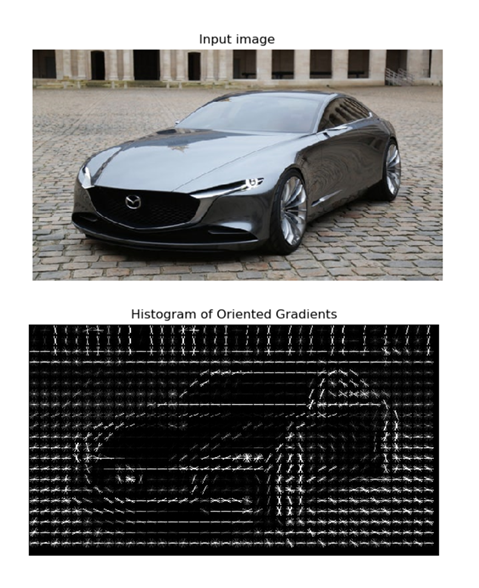
\includegraphics[height=0.9\linewidth]{HOG}
	\caption{Kết quả trích xuất đặc trưng HOG}
	\label{fig:hog}
\end{figure}
\subsubsection{Thu thập tất cả các biểu đồ cường độ gradient định hướng để tạo ra feature vector cuối cùng}
Feature Vector cuối cùng sẽ là tổng của các vector của mỗi block.

\subsection{Bộ dữ liệu huấn luyện}
Bộ dữ liệu được xây dựng từ các ảnh về xe tham gia giao thông trên đường phố Việt Nam, mỗi ảnh có kích thước 64x64 pixels.Ngoài tập dữ liệu dành cho nhận diện, bộ dữ liệu về background và các đối tượng nền cũng cần được thu thập.
\begin{figure}[ht]
	\centering
	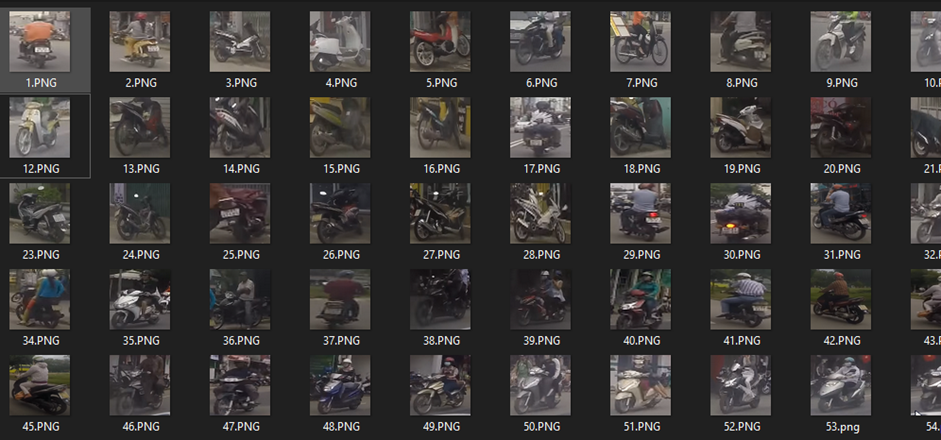
\includegraphics[width=\ScaleIfNeeded]{data}
	\caption{Tập dữ liệu mẫu cho xe máy}
	\label{fig:data}
	\centering
	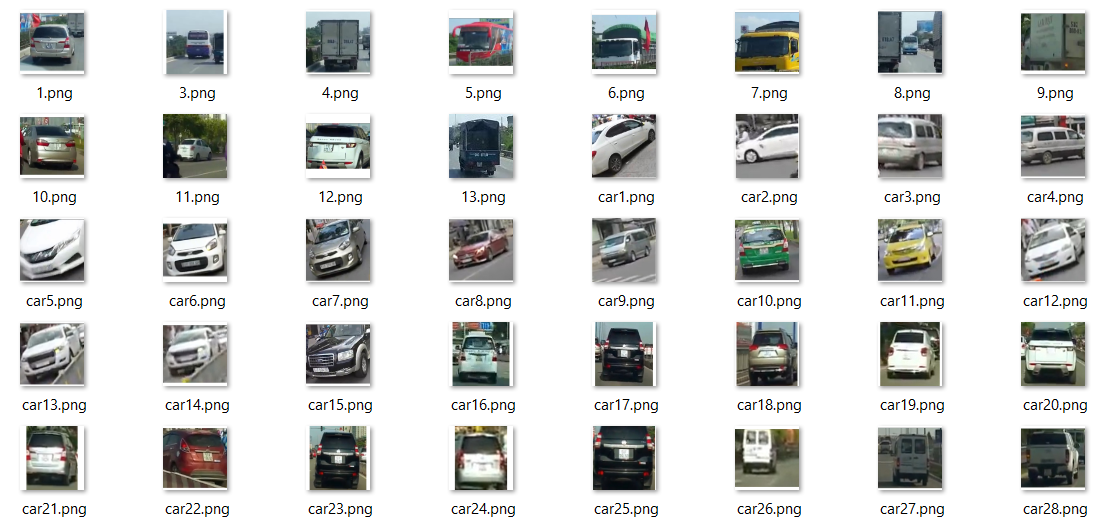
\includegraphics[width=\ScaleIfNeeded, height=0.5\linewidth]{data3}
	\caption{Mẫu dữ liệu cho xe ô tô}
	\label{fig:data3}
	\centering
	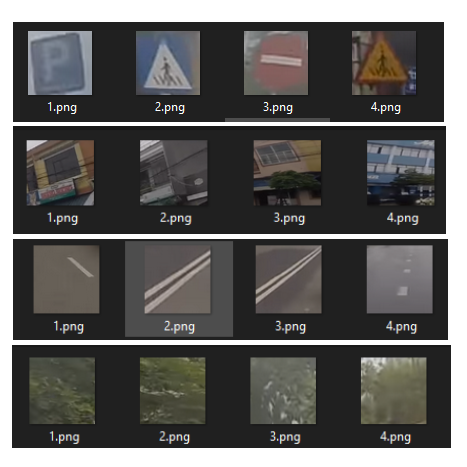
\includegraphics[width=\ScaleIfNeeded,height=0.8\linewidth]{data2}
	\caption{Mẫu dữ liệu nền để loại bỏ trong quá trình nhận diện}
	\label{fig:data2}
\end{figure}

\begin{figure}[ht]
	
\end{figure}

\subsection{SVM (Support Vector Machine) Classifier}
Ý tưởng chính của thuật toán Support Vector Machine (SVM) là tìm được mặt phẳng phân chia 2 lớp dữ liệu, sao cho cách đều 2 (hoặc nhiều) điểm dữ liệu gần nhau nhất của 2 lớp, khoảng cách từ 2 điểm gần nhất đến mặt phẳng phân chia gọi là margin (lề), mục tiêu là tìm được mặt phân chia sao cho margin là lớn nhất. \cite{machinelearning}

\begin{figure}[ht]
	\centering
	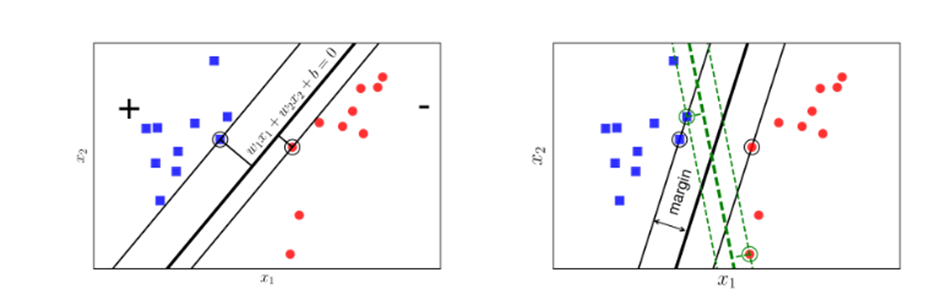
\includegraphics[width=\ScaleIfNeeded, height=0.6\linewidth]{svm}
	\caption{Margin của hai lớp dữ liệu là bằng nhau và lớn nhất có thể}
	\label{fig:svm}
\end{figure}

Như vậy bài toán sẽ được biểu diễn dưới dạng toán học như sau:
Khoảng cách từ một điểm x0 tới mặt phân chia wTx + b = 0 được xác định bởi\\
\[\frac{{\left| {{w^T}{x_0} + b} \right|}}{{{{\left\| w \right\|}_2}}}\]
Giả sử nhãn của mỗi điểm dữ liệu được xác định bởi \[{y_{_i}} = 1\] hoặc \[{y_{_i}} =  - 1\] (class 2)
Với cặp dữ liệu (xn,yn) bất kỳ, khoảng cách từ điểm đó tới mặt phân chia là:


\[\frac{{{y_n}\left( {{w^T}{x_n} + b} \right)}}{{{{\left\| w \right\|}_2}}}\]
Điều này có thể dễ nhận thấy vì theo giả sử ở trên, yn luôn cùng dấu với phía của xn. Từ đó suy ra ${y_n}$ cùng dấu với ${w^T}{x_n} + b$, và tử số luôn là 1 số không âm.
Với mặt phần chia như trên, margin được tính là khoảng cách gần nhất từ 1 điểm tới mặt đó (bất kể điểm nào trong hai classes):
\[margin = \mathop {\min }\limits_n \frac{{{y_n}\left( {{w^T}{x_n} + b} \right)}}{{{{\left\| w \right\|}_2}}}\]


Theo mục đích bài toán, chúng ta cần tìm w và b sao cho margin lớn nhất, tức là
\[\begin{array}{l}
\left( {w,b} \right) = \arg \max \left\{ {\mathop {\min }\limits_n \frac{{{y_n}\left( {{w^T}{x_n} + b} \right)}}{{{{\left\| w \right\|}_2}}}} \right\}\\
\,\,\,\,\,\,\,\,\,\,\,\,\, = \arg \mathop {\max }\limits_{w,b} \left\{ {\frac{1}{{{{\left| {\left| w \right|} \right|}_2}}}\mathop {\min }\limits_n {y_n}\left( {{w^T}{x_n} + b} \right)} \right\}\,\,\,\,\left( 1 \right)
\end{array}\]
Không mất tính tổng quát, ta có thể giả sử: ${y_n}\left( {{w^T}{x_n} + b} \right) = 1$ với những điểm nằm gần mặt phân chia nhất.\\

Như vậy, với mọi n, ta có: $ {y_n}\left( {{w^T}{x_n} + b} \right) \ge 1 $
Vậy bài toán tối ưu (1) có thể đưa về bài toán tối ưu có ràng buộc sau đây:

\[\left( {w,b} \right) = \arg \max \frac{1}{{{{\left\| w \right\|}_2}}}\]
\[subject\,\,to:\,\,\,{y_n}\left( {{w^T}{x_n} + b} \right) \ge 1,\,\,\forall n = 1,2,..,N\,\,\,\,\left( 2 \right)\]\\
Bằng 1 biến đổi đơn giản, ta có thể đưa bài toán này về bài toán dưới đây
\[\begin{array}{l}
\left( {w,b} \right) = \arg \mathop {\min }\limits_{w,b} \frac{1}{2}{\left\| w \right\|_2}^2\\
subject\,\,to:\,1 - {y_n}\left( {{w^T}{x_n} + b} \right) \le 0,\,\forall n = 1,2,..,N\,\,\,\left( 3 \right)
\end{array}\]
Ở đây, chúng ta đã lấy nghịch đảo hàm mục tiêu, bình phương nó để được một hàm khả vi, và nhân với 1/2 để biểu thức đạo hàm đẹp hơn.
Để tìm nghiệm của bài toán này, ta sử dụng phương pháp nhân tử Lagrange. Tuy nhiên, việc giải bài toán này trở nên phức tạp khi số chiều d của không gian dữ liệu và số điểm dữ liệu N tăng lên cao. Thực tế, người ta thường giải bài toán này bằng bài toán đối ngẫu. Thứ nhất, bài toán đối ngẫu có những tính chất thú vị hơn khiến nó được giải hiệu quả hơn. Thứ hai, trong quá trình xây dựng bài toán đối ngẫu, người ta thấy rằng SVM có thể được áp dụng cho những bài toán mà dữ liệu không linearly separable, tức các đường phân chia không phải là một mặt phẳng mà có thể là các mặt có hình thù phức tạp hơn.



\subsection{Sliding Window}
Sau khi huấn luyện xong bộ phân loại (classifier), bước tiếp theo chúng ta sẽ làm đó là áp dụng bộ phân loại này lên từng phần của 1 bức ảnh để có thể xác định được vị trí của vật cần nhận diện (xe máy hay ô tô). \cite{harveen}

Cửa sổ trượt (sliding window) là kỹ thuật mà ta dùng 1 cửa sổ (window, hay tên gọi khác là kernel) để trượt trên mỗi pixel của ảnh. Tại mỗi pixel trong quá trình trượt, ta áp dụng phép biến đổi giữa các pixel trên cửa sổ và các pixel tương ứng trên vùng ảnh.

Một vấn đề quan trọng cần đặt ra đó là chọn kích thước của cửa sổ, bởi vì trong một bức hình, sẽ có những vật thể ở phía xa và phía gần, do đó kích thước của chúng trên bức hình sẽ không giống nhau, ta phải chọn nhiều kích thước cửa sổ thì mới có thể xác định được chính xác và đầy đủ nhất các vật thể.

Ví dụ như bức hình dưới đây, ta chọn các kích thước cửa sổ cũng như độ chồng lặp giữa các cửa sổ liên tiếp ứng với mỗi phần của bức hình:
\begin{figure}[ht]
	\centering
	\includegraphics[width=\ScaleIfNeeded]{"window sizes"}
	\caption{Các kích thước cửa sổ ứng với vùng hoạt động của nó trên một bức hình}
	\label{fig:window-sizes}
\end{figure}
\begin{figure}[ht]
	\centering
	\includegraphics[width=\ScaleIfNeeded]{"sliding window"}
	\caption{Minh hoạ sliding window}
	\label{fig:sliding-window}
\end{figure}

Sau khi đã xác định kích thước của các cửa sổ, ta tiến hành trượt chúng trên bức ảnh để nhận dạng ra vật thể (xe máy, ô tô), lưu ý rằng mẫu huấn luyện của chúng ta có kích thước 64x64 pixel, nên đối với các cửa sổ không cùng kích thước trên, ta phải resize lại thành 64x64 pixel.
\subsection{Bounding Object}
Sau khi sử dụng cửa sổ trượt, ta có thể xác định được vị trí vật thể, vấn đề tiếp theo đặt ra là làm sao có thể vẽ được một khung bao quanh vật thể (bounding box), Heatmap có thể giúp ta giải quyết vấn đề này. \\
Đầu tiên, tạo một bức ảnh trống màu đen (blank black image) có cùng kích thước với bức hình gốc, tại các cửa sổ mà được xác định là chứa vật thể, ta sẽ cộng giá trị của các điểm ảnh trong cửa sổ này lên 1. Theo cách này, chúng ta sẽ có các vùng có cường độ khác nhau và vùng chứa vật thể chính là vùng có cường độ mạnh nhất.Dưới đây là hình minh hoạ việc sử dụng heatmap để vẽ bounding box.
\begin{figure}[ht]
	\centering
	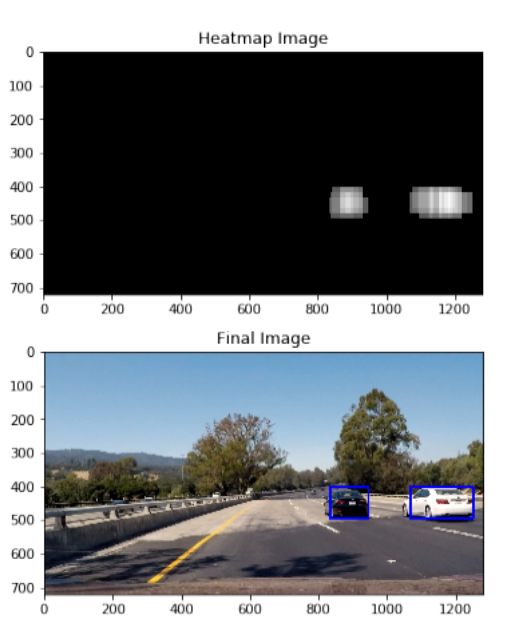
\includegraphics[width=\ScaleIfNeeded]{heatmap2}
	\caption{Dùng heatmap để xác định bounding box cho object}
	\label{fig:heatmap2}
\end{figure}

\section{KẾT QUẢ}
\label{Sec:KetQuaMoPhong}
%
Trong phần này, nhóm sẽ thiết lập chương trình mô phỏng bằng Python để kiểm chứng các kết quả phân tích ở phần trên. 
Với stepsize =0.3, thuật toán nhận diện khá chính xác, tuy nhiên vẫn có một số trường hợp nhận dạng sai vì dữ liệu huấn luyện chưa đủ lớn.

\begin{figure}[!h]
	\centering
	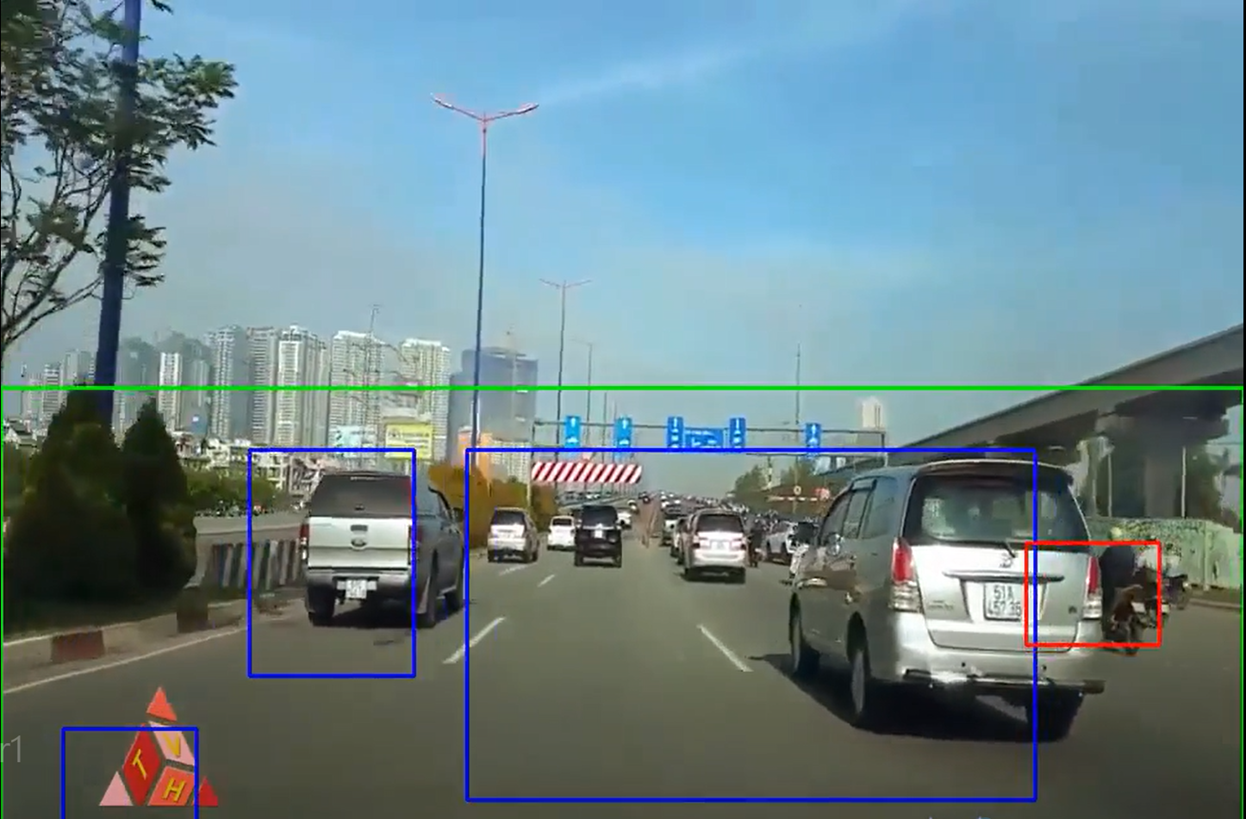
\includegraphics[width=\ScaleIfNeeded, height=0.3\linewidth]{ketqua1}
	\caption{Kết quả nhận diện với stepsize=0.3}
	\label{fig:ketqua1}
\end{figure}
\begin{figure}[h]
	\centering
	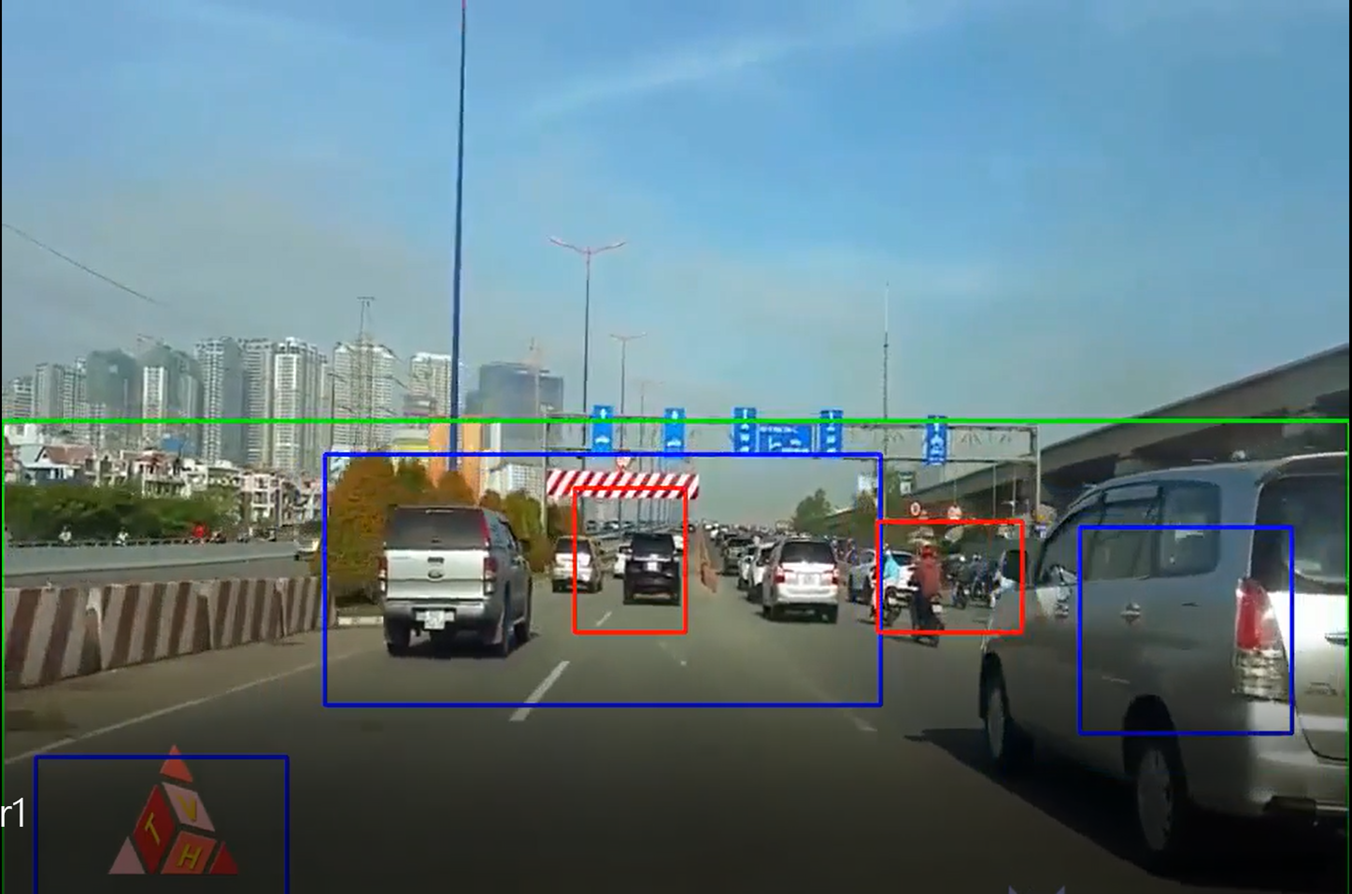
\includegraphics[width=1\linewidth, height=0.2\textheight]{ketqua2}
	\caption{Trường hợp nhận dạng nhầm xe máy thành ô tô}
	\label{fig:ketqua2}
\end{figure}

Với stepsize=0.2, ta thấy đường bao lớn hơn. Lý do là vì bước nhảy nhỏ hơn tạo ra nhiều khung, sau đó heatmap gộp các khung này lại tạo thành khung lớn
\begin{figure}[h]
	\centering
	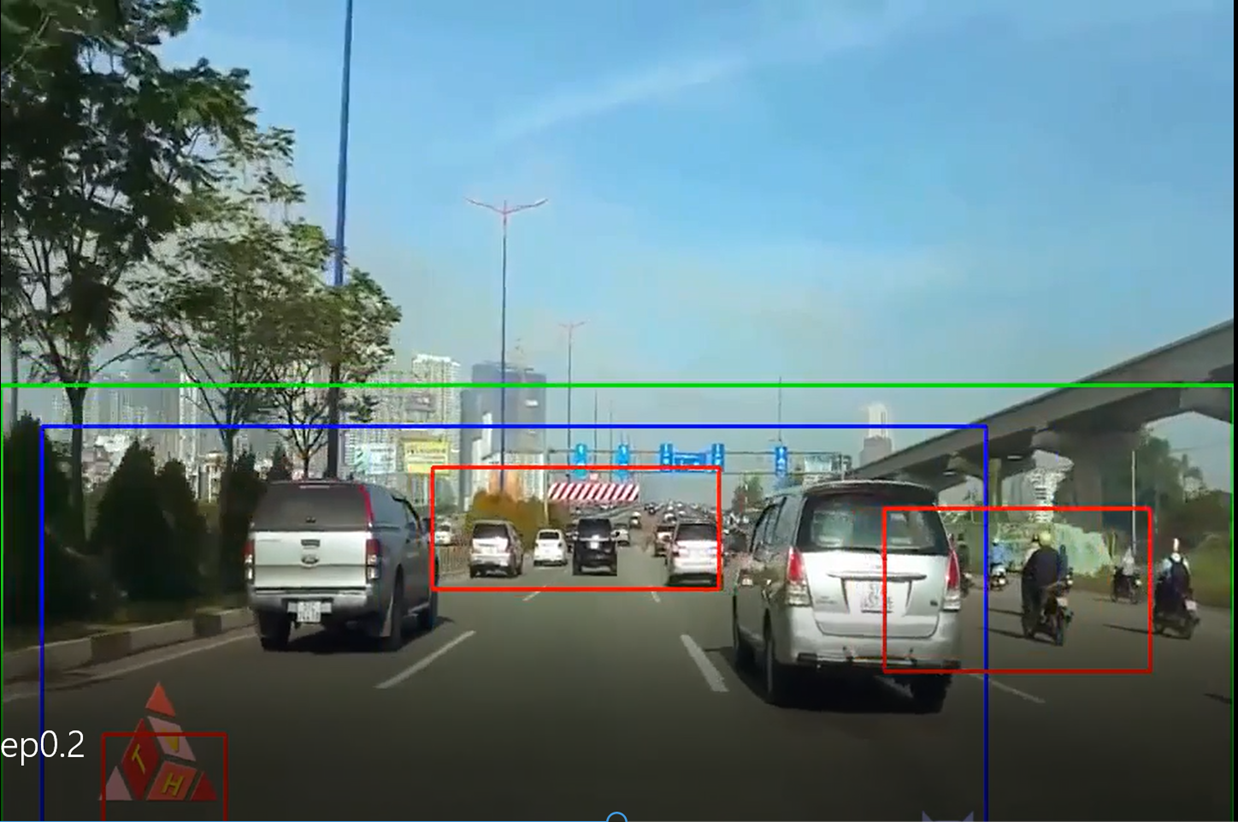
\includegraphics[width=1\linewidth, height=0.2\textheight]{ketqua3}
	\caption{Kết quả nhận diện với stepsize=0.2}
	\label{fig:ketqua3}
\end{figure}

Stepsize=0.4, bước nhảy lớn thì sẽ không xác định được xe máy, do kích thước chiều ngang của người đi xe máy khá nhỏ

\begin{figure}[h]
	\centering
	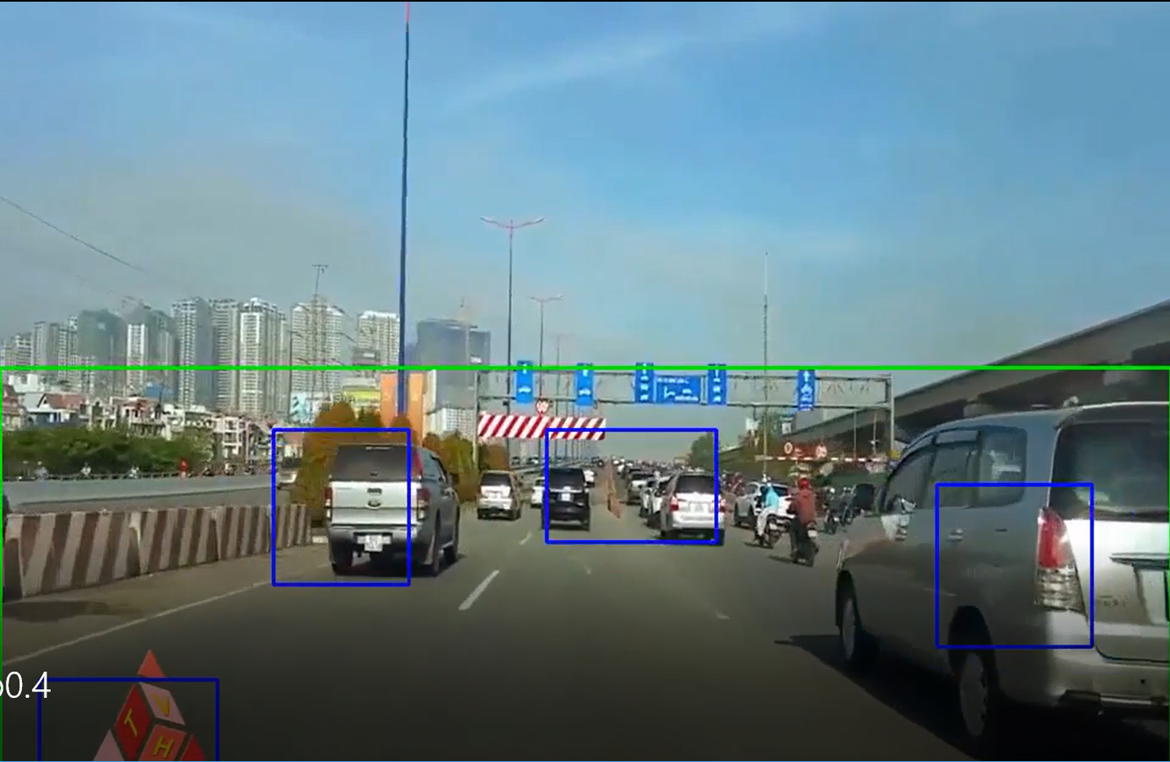
\includegraphics[width=1\linewidth, height=0.2\textheight]{ketqua4}
	\caption{Kết quả với stepsize=0.4}
	\label{fig:ketqua4}
\end{figure}


\pagebreak


\section{KẾT LUẬN}
\label{Sec:KetLuan}
Phương pháp HOG là phương pháp trích xuất đặc trưng giúp giảm số chiều của dữ liệu -> hiệu quả về tốc độ tính toán.
Thuật toán SVM là thuật toán cho kết quả phân loại tốt.
Kết quả thực hiện tốt, tuy nhiên vẫn có trường hợp nhận dạng sai do database chưa đủ lớn.
Chưa có sự tối ưu về mặt thời gian và kích thước đường bao.






\section*{LỜI CẢM ƠN}
Để có được bài nghiên cứu này, nhóm xin cảm ơn Thầy Đặng Nguyên Châu đã hỗ trợ rất nhiều về các kiến thức về xử lý ảnh cũng như các phương pháp phân loại, ngoài ra thầy cũng tạo điều kiện thuận lợi để nhóm có thời gian làm bài báo cáo được tốt hơn.
{\Large 
\bibliographystyle{IEEEtran}

\bibliography{reference}
}

\end{document}


